\section{Literature Review} 
\label{sec:litreview}
The exploration and documentation of caves underpins developments in the natural sciences, geographic databases, and conservation of subterranean fauna (Kambesis 2009; Bichuette \& Trajano 2018). Historically, researchers have been constrained by dangerous or otherwise inaccessible cave features such as vertical drops and tight areas. Recent improvements in robotic technologies and their accessibility presents an opportunity to expand cave exploration capabilities (Dubowsky et al 2005). This literature review initially explores mapping and localisation technologies often implemented into robotic systems to determine which is most appropriate for the CaveX prototype. This analysis builds upon the conclusions of the 2022 CaveX team's literature review through a deeper assessment of SLAM algorithms and their analogous counterparts. Next, approaches to obstacle detection, avoidance, and pathfinding are considered in the context of the unique challenges imposed by caves. Finally, a review of gait optimisation strategies is conducted with consideration to its implementation with obstacle detection, avoidance, and pathfinding.

\subsection{Mapping \& Localisation}

In robotics, mapping and localisation are the processes by which a robot constructs a representation of its environment and determines its location within an environment, respectively. Thus, SLAM is a process wherein a robot determines where it is located within its local environment while constructing a map of such environment (Mur-Artal, Montiel \& Tardós 2015). Real time SLAM algorithms are attractive for systems requiring autonomous navigation due to a lack of reliance on outside data such as Global Navigation Satellite System (GNSS) information (Auat Cheein et al. 2010). The 2022 CaveX team determined that visual SLAM methods are unsuitable for cave exploration due to the presence of photosensitive fauna and flora. These methods would present a challenge in balancing the need for data to conduct SLAM with minimising damaging effects to cave inhabitants (Bright et al. 2022; Williams 2021). This, therefore, necessitates the implementation of LiDAR-based SLAM. 

While there are several algorithms for SLAM using LiDAR, a common high-performance algorithm is the LiDAR Odometry and Mapping (LOAM) algorithm (Abdelaziz \& El-Rabbany 2022). At a high level, it works by running two algorithms: one high-frequency but low-fidelity odometry algorithm to estimate robot velocity and one higher fidelity but lower frequency algorithm which determines the spatial transform between two LiDAR point clouds. The process of determining this spatial transform is known as matching. Separating these two functions facilitates reduced computational load at the expense of extremely high accuracy (Zhang \& Singh 2014). Subsequent to LOAM's publication, improved variants such as Advanced LOAM (A-LOAM), Lightweight and Ground-Optimised LOAM (LeGO-LOAM), and Fast LOAM (F-LOAM) have been developed to provide improved performance (Abdelaziz \& El-Rabbany 2022). A-LOAM focuses on general computational optimisation through the removal of redundant operations (Qin \& Cao 2019). LeGO-LOAM targets computational performance and algorithm accuracy improvements for LOAM application in ground vehicles by windowing point clouds before analysis and reducing noise in data (Shan \& Englot 2018). F-LOAM improves computational performance through a dynamic combination of feature extraction, distortion compensation, pose optimisation, and mapping. By assuming that the time between consecutive LiDAR scans is small, the linear and angular velocities in that time are assumed to be constant. This allows the distortion in a scan to be partially corrected by inferring the LiDAR scanner's motion between the two scans. Then, after pose estimation, the distortion is re-computed to update the final map (Wang et al. 2021). In contrast, A-LOAM and LeGO-LOAM's brute force iterative approaches to distortion compensation require greater computational resources. However, their approach avoids error due to variable linear and angular velocities between scans (Qin \& Cao 2019; Shan \& Englot 2018). Experimentally, Wang et al. (2021) showed that LeGO-LOAM has the smallest computational cost of LOAM, A-LOAM, LeGO-LOAM, and F-LOAM. However, LeGO-LOAM exhibited the highest average translational error (ATE) and average rotational error (ARE). At an ATE, ARE, and computing time of 0.80\%, 0.0048deg/m, and 80ms, respectively,  F-LOAM exhibits approximately 1.9 times less error than LeGO-LOAM in translation, 2.4 times less error in rotation, and is 12.5\% slower. F-LOAM also outperformed LOAM and A-LOAM in all three metrics (Wang et al. 2021). Given the limited computational resources of the CaveX prototype's NVIDIA Jetson Nano, F-LOAM presents the most ideal trade off between computing time and algorithm accuracy. However, all algorithms discussed have been tested on a central processing unit (CPU), which is not the ideal environment for point cloud processing (Wang et al. 2021; Anand et al. 2020). Thus, while porting them to a graphics processing unit (GPU) environment such as the Jetson's CUDA cores is likely to yield a significant reduction in computing time, the exact improvements are unknown.

\subsection{Obstacle Detection \& Avoidance}

Obstacle detection and obstacle avoidance are the phenomena wherein a system can identify obstacles in its path and make the appropriate adjustments to prevent a collision while continuing to accomplish the system's objective(s). Therefore, solving these problems is critical to producing a system which is autonomy-capable. Obstacles can be broadly categorised as either positive or negative: positive obstacles are those which protrude up from the ground or otherwise physically impede a path, whereas negative obstacles are voids in the ground such as ditches, pits, or downward-sloped terrain (Shang et al. 2015, p. 591). Further classification of obstacles is to describe them as either static or dynamic, where static obstacles are stationary and dynamic obstacles are moving (Asvadi et al. 2016). This section describes and discusses existing LiDAR-based obstacle detection and avoidance methods to assess their utility in cave exploration.

Typically, obstacle detection is conducted using a sensor fusion approach with data from LiDAR or Radio Detection and Ranging (RADAR) combined with stereo and monocular cameras, inertial measurement units (IMUs), and GPS sensors. This is because much of the existing work done to tackle the problem is in the field of autonomous driving and advanced driver assistance systems (Badue et al. 2021; Asvadi et al. 2016). However, existing research has developed algorithms for LiDAR-only obstacle detection. One approach is to segment the ground surface from the overall LiDAR point cloud before voxelising the remaining obstacle point cloud for further static and dynamic obstacle segmentation. Due to the sparse and non-uniform nature of LiDAR point clouds, an interquartile range (IQR) gating strategy and random sample consensus (RANSAC)-based plane fitting is employed to minimise the impact of outliers. This algorithm showed promising results as it missed only 6.18\% of obstacles and had a false-positive rate of 3.09\%.  (Asvadi et al. 2016). Critically, it conducts point cloud preprocessing in a manner similar to that of SLAM algorithms and, therefore, it may be possible to integrate them to reduce overall computational load. However, this method does not detect negative obstacles and therefore would need to be combined with an algorithm that does to be suitable for cave exploration. A lack of literature on combined algorithms means additional work is required to determine an integration technique.

An alternative approach is a dynamic clustering algorithm which identifies objects through spatial clustering techniques. The approach developed by Gao, Li \& Zhang (2021) builds upon previous findings regarding density-based spatial clustering (DSC) of applications with noise by accounting for the point cloud sparsity increase with distance from the sensor. This algorithm showed a true positive detection rate of 85.66\% and a false negative rate of 5.98\%. However, it suffers from the same issue as the previous algorithm in that it cannot detect negative obstacles (Gao, Li \& Zhang 2021).

While previously-discussed algorithms have been based on hard-coded mathematical filters and geometric criteria, an emerging method of obstacle detection is applying deep learning techniques. Two deep learning models for point cloud classification and segmentation are PointNet and SECOND. PointNet focuses on object classification, part segmentation, and semantic segmentation whereas SECOND targets object and direction classification (Qi et al. 2017; Yan, Mao \& Li 2018). Deep learning methods show promise for obstacle detection but are often inaccessible or suboptimal due to the specialised expertise needed, high-performance hardware required for training the models, or their non-deterministic nature rendering them a high risk endeavour. However, the SECOND model was trained in 19 hours on a single consumer NVIDIA GTX 1080Ti (Yan, Mao \& Li 2018). Hence, if the two former issues can be overcome, then application of the model in a cave environment may be possible. One potential method to overcome the model's non-deterministic nature is to fuse it with a deterministic algorithm. However, this area is lacking in research.  

Obstacle avoidance is dependent on obstacle data but can be independent of the algorithm used to acquire such data. A quintessential real time obstacle avoidance technique is the artificial potential field method developed by Khatib (1986). This method involves the construction of a model wherein virtual attractive and repulsive forces are produced by the goal location and the obstacles in the field, respectively. By applying an iterative approach where each iteration is triggered by the movement of a robot, the optimal path vector at the robot's position during the iteration can be determined. Thus, across a series of iterations, the robot can reach its goal position while avoiding obstacles in its path.

\subsection{Pathfinding}
In general, pathfinding is the process of determining the optimal path to take in space given a set of conditions (Le et al. 2018). Pathfinding algorithms can be categorised as global or local. Global pathfinding algorithms rely on complete data of the paths and obstacles in an environment, whereas local algorithms find a path from real time sensor data (Kim et al. 2018; Le et al. 2018). By definition, exploration robots are constrained by a lack of data and, therefore, rely on local pathfinding algorithms to navigate. A unique consideration of exploration robotics is that the system should prioritise unexplored paths over explored ones. Additionally, it should be capable of returning to its starting position via the path it originally took. Thus, existing local pathfinding algorithms are explored to examine their viability for cave exploration.

A modified version of the rapidly-exploring random tree (RRT) algorithm, executive rapidly-exploring random tree (ERRT), was implemented into a robot snake to facilitate LiDAR-based pathfinding. This algorithm involves setting a goal position before an iterative brute force approach is taken to find a path between the robot's current position and its goal. This approach can be effective, but its brute force nature means the computational load grows extremely fast with distance to the goal position. This trend is due to the growth in the number of possible paths and the number of vertices within a path which, therefore, increases the number of states for the iterator to consider (Yang, Wang \& Shen 2020; LaValle \& Kuffner 2001). 

A SLAM-based pathfinding algorithm for construction applications involves applying the artificial potential field method developed by Khatib (1986) based on the results of an obstacle detection algorithm to determine the optimal path to the goal position. By iteratively applying the Newton direction method while a robot moves, the optimal path vector at that location can be determined. As the robot approaches the goal position, the goal position can be re-allocated based on new sensor information or it can remain the same depending on what is most appropriate for the situation (Kim et al. 2018). Additionally, due to the artificial potential field method's virtual force behaviour, negative obstacles can be accounted for in the path planning process. However, such an implementation relies on the ability to detect such obstacles. Hence, detection is the major limitation of this algorithm.

The primary limitation of pathfinding algorithms in robotics, such as RRT, ERRT, and the artificial potential field method, is a lack of consideration of a robot's kinematic constraints; the algorithms focus solely on the generation of a path without obstacles. Limited literature in this area means that a custom algorithm would need to be developed wherein a kinematic model of the robot predicts its kinematic state at future iterations of a path and adjusts the path accordingly.

\begin{figure}[H]
    \centering
    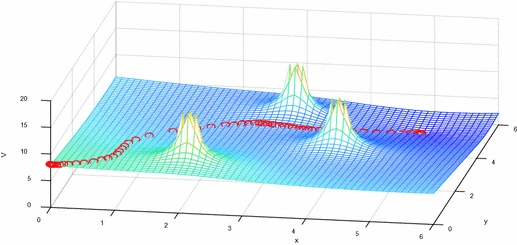
\includegraphics[scale=0.6]{images/artificialPotentialField.png}
    \caption{Example artificial potential field and the resulting optimal path trajectory (Kim et al. 2018)}
    \label{fig:artifical_potential_field}
\end{figure}

\subsection{Dynamic Gait Optimisation}

The goal of dynamic gait optimisation in quasi-static multi-legged robots, such as a hexapod, is to improve their real time adaptability and stability in challenging terrain. This ability is of particular importance in cave exploration as cave surfaces are often non-uniform and unpredictable (Novak et al. 2021). This section explores existing gait optimisation algorithms to assess their suitability to a cave-exploring hexapod.

Previously, a basic style of gait optimisation in quadrupedal and hexapod robots has been to ensure its body is aligned with the terrain plane and its height kept constant. The primary issue with this technique is a lack of consideration to spatial constraints. Tight spaces and non-uniform terrain can result in a failure. Thus, this technique alone is suboptimal for unpredictable cave terrain (Chen, Liu \& Gan 2022; Bartsch et al. 2012). Chen, Liu \& Gan (2022) found that employing a minimisation and pseudo-inverse optimisation technique improved a six-legged robot's walking speed by 17.1\% and adaptability in slopes and steps by 48.5\% and 96.0\%, respectively. However, their robot structure, while six-legged, was different to the current CaveX prototype in that each leg is comprised of three sub-legs. Despite this, their kinematic analysis may be ported to an appropriate structure.

An alternative approach to gait optimisation is to directly measure the force applied to each of robot's feet. The Foot Force Stability Margin (FFSM) was developed to serve as a force-based test to assess a system's stability. Its low computational cost and sensitivity make it attractive for real time applications. However, its simplicity constrains it to act as an indicator of stability rather than a process to achieve stability. Subsequently, the Modified Foot Force Stability Margin (MFFSM) was developed to build upon FFSM by taking robot geometry and top-heaviness into account (Agheli \& Nestinger 2012). Thus, MFFSM could be used to form an iterative stability algorithm wherein a robot's centre of gravity is lowered to increase stability when a low-stability state is detected. This process, however, may be suboptimal as it has only one course of action to correct a low-stability state.

More complex techniques fuse advanced forward and inverse kinematic analysis or artificial intelligence with sensor feedback to facilitate dynamic terrain compensation. One such algorithm involves using a dynamic model, motor torque feedback, and locomotion state information to iteratively adjust the endpoint positions of legs being lowered such that they account for ground surface inconsistencies (Zangrandi, Arrigoni \& Braghin 2021). While this approach shows promising results, its complexity and reliance on a terrain elevation function present significant development challenges. An alternative approach is to implement a reinforcement learning (RL) algorithm which provides a control system with the ability to learn via trial and error. In one approach, a Spiking Neural Network (SNN) took visual and gyroscopic input to learn gait optimisations via determining whether stability was lost during a movement and factoring that into its reward function. The SNN frequently converged with the target gait pattern but, at a median of 207 iterations for convergence, spent considerable time learning (Lele et al. 2020). While RL has significant potential for future applications, its inherent stochastic nature significantly increases the expertise required for development and risk to the robot during its operation.

Overall, of the gait optimisation approaches discussed, the algorithm developed by Zangrandi, Arrigoni \& Braghin (2021) provides the best combination of dynamic capability and algorithmic determinism. However, this comes at the cost of complexity. FFSM and MFFSM are attractive due to their simplicity but this simplicity also constrains the resulting algorithms. The approach adopted by Chen, Liu \& Gan (2022) shows considerable improvements but for an alternative hexapod morphology. RL-based algorithms have the potential yield impressive dynamic capabilities but require considerable expertise to optimise.

\subsection{Findings}
The findings from the literature review are summarised in Table \ref{tab:lit_review_outcomes}. The advantages and disadvantages of different solutions to implement the project's technical objectives are compared for a variety of different sources.
\newpage
\bgroup

    \centering
    \begin{xltabular}{\textwidth}{|
    >{\hsize=.6\hsize\RaggedRight}X|% 10% of 4\hsize 
    >{\hsize=0.8\hsize\RaggedRight}X|% 30% of 4\hsize
    >{\hsize=1.4\hsize\RaggedRight}X|% 30% of 4\hsize 
    >{\hsize=1.2\hsize\RaggedRight}X|% 30% of 4\hsize
       % sum=4.0\hsize for 4 columns
  }
    \caption{Potential solutions identified in literature organised by theme.}
    \\ \hline
    \rowcolor{gray!50}
    \textbf{Theme} & \textbf{Source} & \textbf{Summary} & \textbf{Outcome}
    \\ \hline
    % \csvreader[late after line = \\, separator = semicolon]{./csv/abbreviations.csv}{1 = \a, 2 = \b}{\a & \b}
    
    \multirow{3}{=}{Mapping \& Localisation} & Qin \& Cao 2019 & A-LOAM underperforms compared to LeGO-LOAM and F-LOAM & \multirow{3}{=}{F-LOAM is the most appropriate SLAM algorithm given the computational constraints} \\
    \Cline{1pt}{2-3}
    & Shan \& Englot 2018 & LeGO-LOAM requires the least computational power but produces the most error &\\
    \Cline{1pt}{2-3}
    & Wang et al. 2021 & F-LOAM provides the best balance of accuracy and computational resources &\\

    \hline
    
    \multirow{4}{=}{Obstacle Detection \& Avoidance} & Asvadi et al. 2016 & Statistical RANSAC approach identified 94\% of obstacles but cannot detect negative obstacles & \multirow{4}{=}{The statistical RANSAC approach to obstacle detection and the Artificial Potential Field Method are the optimal techniques for obstacle detection and avoidance} \\
    \Cline{1pt}{2-3}
    & Ghao, Li \& Zhang 2021 & TP rate of 85\% but cannot detect negative obstacles & \\
    \Cline{1pt}{2-3}
    & Qi et al. 2017 & PointNet can perform object classification but is complicated and non-deterministic &\\
    \Cline{1pt}{2-3}
    & Yan, Mao \& Li 2018 & SECOND can perform object and direction classification but is complicated and non-deterministic &\\

    \hline
    
    \multirow{2}{=}{Pathfinding} & Yang, Wang \& Shen 2020; LaValle \& Kuffner 2001 & Effective but computationally expensive & \multirow{2}{=}{The Artificial Potential Field Method is the best approach as it allows for iterative updating of the ideal velocity vector and limits brute forcing a path} \\
    \Cline{1pt}{2-3}
     & Khatib 1986; Kim et al. 2018 & Works for positive and negative obstacles, computationally cheap & \\

    \hline
    
    \multirow{3}{=}{Dynamic Gait Optimisation} & Chen, Liu \& Gan 2022 & Effective but for a different hexapod anatomy & \multirow{3}{=}{The dynamic model developed by Zangrandi, Arrigoni \& Braghin (2021) provides the optimal combination of capability and determinism in gait optimisation } \\
    \Cline{1pt}{2-3}
    & Agheli \& Nestinger 2012 & Too basic for a cave environment &\\
    \Cline{1pt}{2-3}
    & Zangrandi, Arrigoni \& Braghin 2021 & Effective and for the appropriate hexapod anatomy &\\
    \Cline{1pt}{2-3}
    & Lele et al. 2020 & Somewhat effective but experimental and stochastic &\\
    \hline
    \end{xltabular}
    \label{tab:lit_review_outcomes}
\egroup